 % Drawing angles using the PG 3.0 angles and quotes libraries
% Author: Paul Gaborit
\documentclass[tikz,border=10pt]{standalone}
\usetikzlibrary{quotes,angles}
\begin{document}
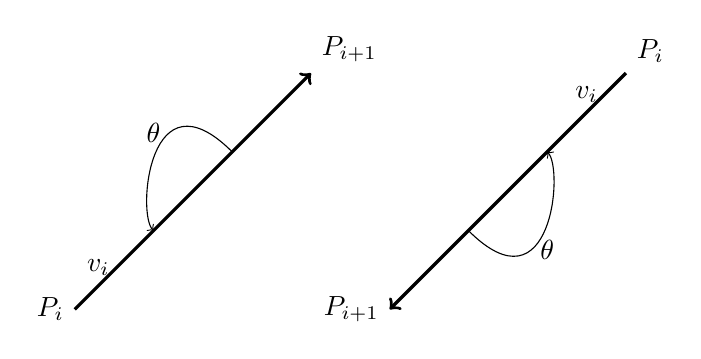
\begin{tikzpicture}
  \draw
    [->, very thick](0,0) coordinate (b) node[left] {$P_i$}
    -- (3,3) coordinate (c) node[above right] {$P_{i+1}$};
  \draw [->](2,2) .. controls +(135:1.5cm) and +(135:0.3cm) .. (1,1);
  \node[above] at (1,2) {$\theta$};
  \node[above] at (0.3,0.3) {$v_i$};
  \draw
    [->, very thick](7,3) coordinate (b1) node[above right] {$P_i$}
    -- (4,0) coordinate (c1) node[left] {$P_{i+1}$};
  \draw [->](5,1) .. controls +(315:1.5cm) and +(315:0.3cm) .. (6,2);
  \node[below] at (6,1) {$\theta$};
  \node[above] at (6.5,2.5) {$v_i$};
\end{tikzpicture}
\end{document}

